% Discuss the PUF ROK and how it is relevant

\chapter{Read Once Keys}
\label{chapter:rok}

\section{Overview}
In this section, we present the definition, design, and implementation of read-once keys (ROKs). The presentation is this chapter
follows after~\cite{PUFROK}.

The term read-once key (ROK) describes the abstract notion that a cryptographic key can be read and used for encryption
and decryption only once. While it seems intuitive that a trusted piece of software could be designed that deletes a key right after
using it, such a scheme na\"{i}vely depends on the proper execution of the program. This approach could be easily
circumvented by running the code within a debugging environment that halts execution of the code before the deletion occurs.
That is, the notion of a ROK entails a stronger protection method wherein the process of reading the key 
results in its immediate destruction.

ROKs could be applied in a number of interesting scenarios. One application could be to create one-time programs~\cite{otp},
which could be beneficial for protecting the intellectual property of a piece of software. A potential client
could download a fully functional one-time program for evaluation before committing to a purchase.  A similar application
would be self-destructing email.  In that case, the sender could encrypt a message with a ROK; the message would then
be destroyed immediately after the recipient reads the message.  More generally, there is considerable interest in self-destructing
data, both commercially~\cite{ironkey} and academically~\cite{vanish}.  In addition, the use of trusted hardware tokens have been
proposed for applications including program obfuscation~\cite{obfusc}, monotonic counters~\cite{monotonictpm}, oblivious
transfer~\cite{ottamper}, and generalized secure computation~\cite{tamperhw}.  ROKs can provide the required functionality
for these applications.

Another interesting application of PUF ROKs is to defend against physical attacks on cryptographic protocols.  For example,
consider fault injection attacks on RSA~\cite{rsapub,pertrsa,insecrsa,rsaltr,fault}.  In these attacks, the algorithm is repeatedly executed
with the same key, using a controlled fault injection technique that will yield detectable differences in the output.  After enough such
iterations, the attacker is able to recover the key in full.  Similarly, ``freezing'' is another class of physical attack
that can extract a key if it was \emph{ever} stored in an accessible part of memory~\cite{freezing}.  PUF ROKs offer a unique defense against
all of these attacks because repeated execution with the same key cannot occur, and the key is \emph{never} actually present
in addressable physical memory.

The ability to generate ROKs in a controlled manner could also lead to an extension where keys can be generated and used
a multiple, but limited, number of times. For example, consider the use of ROKs to encrypt a public key {\it pk}. If an
identical ROK can be generated twice, the owner of {\it pk} could first use the key to create $e_{ROK}(pk)$ (indicating the
encryption of {\it pk} under with the ROK). Later, an authorized party could create the ROK a second time to decrypt the
key. Such a scheme could be used to delegate the authority to cryptographically sign documents.

In a sense, a ROK is an example of a program obfuscator.  An obfuscator $\mathcal{O}$ takes a program $\mathcal{P}$ as
input and returns $\mathcal{O}(\mathcal{P})$, which is functionally identical to $\mathcal{P}$ but indecipherable.  A ROK,
then, involves an obfuscator that makes only the key indecipherable.  While ROKs are promising ideals, the
disheartening fact is that program obfuscators--of which ROKs are one example--cannot be created through algorithmic
processes alone~\cite{impobf}.  Instead, trusted hardware is required to guarantee the immediate destruction of the
key~\cite{otp}.  However, we are aware of no work that has specifically undertaken the task of designing and creating such
trusted hardware for the purpose of generating a ROK.

Our insight for the design of such ``PUF ROKs'' is to incorporate the PUF in a feedback loop for a system-on-chip
(SoC) design.\footnote{Our design could also be made to work for application-specific integrated circuits (ASICs), but
we limit our discussion to SoC designs for simplicity.} That is, our design is for the PUF to reside on the same chip
as the processor core that performs the encryption. This integration of the PUF and the processor core protects the
secrecy of the key.  An attempt to read the key from memory (given physical access) will fail, because the key \emph{never
exists in addressable memory}.  Also, attempts to learn the key from bus communication will be difficult or
impossible, as each key is used to encrypt only a single message, and the key is \emph{never transmitted across the bus}.

The unpredictable nature of PUFs provides a high probability that each iteration of a ROK generation will produce a
unique, seemingly random key.  Yet, to ensure that a key can be generated to perform both encryption and decryption,
the PUF must be initialized repeatedly to some state, thus providing the same 
sequence of keys.  To accomplish this, Alice could provide an initial seed to produce a sequence of keys that are used to encrypt
a set of secrets. Alice could then reset the seed value before making the device available to Bob. Bob, then, could use the PUF to
recreate the keys in order, decrypting the secrets. As Bob has no knowledge of the seed value, he is unable to reset the
device and cannot recreate the key just used.

Astute readers will note the similarities between our approach and using a chain of cryptographic hashes to generate
keys.  That is, given a seed $x_0$, the keys would be {\sf H}$(x_0)$, {\sf H}({\sf H}($x_0$)), etc., where {\sf H}
denotes a cryptographic hash function.  The insight of our approach is that a PUF, as a trusted piece of hardware,
can provide a hardware-based implementation that is analogous to a hash function, but is more secure than
software implementations of such algorithms.

\section{Read Once Keys (ROK)}
Our formal notion of a ROK is based on an adaptation of Turing machines.  Specifically, define the machine $T$ to be
\begin{center}
\begin{tabular}{c}
$T = < Q,q_0,\delta,\Gamma,\iota >$
\end{tabular}
\end{center}
where $Q$ is the set of possible states, $q_0$ is the initial state, $\delta$ defines the transition
from one state to another based on processing the symbols $\Gamma$, given input $\iota$.  Readers familiar with Turing
machines will note that $\iota$ is new.  In essence, we are dividing the traditional input symbols into code ($\Gamma$)
and data ($\iota$).  For the sake of simplicity, we assume that $\iota$ only consists of messages to be encrypted or
decrypted and ignore other types of input data.  Thus, the definition of $\delta$ is determined by the execution of
instructions $\gamma_1, \gamma_2, \ldots, \gamma_i$, where consuming $\gamma_i \in \Gamma$ results in the transition from state $q_i$ to
$q_{i+1}$.  Based on this formalism, we propose the following primitives.

\begin{itemize}
\item The \emph{\bf encrypt primitive} {\sf Enc}$(\gamma_i,q_i,m)$ encrypts the message $m \in \iota$ given the instruction
$\gamma_i$ and the state $q_i$.  The system then transitions to $q_{i+1}$ and produces the returned value as $e(m)$ as a side effect.
\item The \emph{\bf decrypt primitive} {\sf Dec}$(\gamma_j,q_j,e)$ decrypts the ciphertext $e \in \iota$ given the instruction
$\gamma_j$ and the state $q_j$.  If the decryption is successful, the primitive returns $m$.  Otherwise, the return value is 
denoted $\emptyset$.  The system then transitions to $q_{j+1}$.
\end{itemize}

Informally, $\gamma_i$ and $q_i$ describe the current instruction and the contents of memory for a single execution
of a program, and capture the state of the system just before executing the encrypt or decrypt primitive.  That is,
if the execution of the program is suspended for a brief time, $\gamma_i,q_i$ would describe a snapshot of the
stack, the value stored in the instruction pointer (IP) register, the values of all dynamically allocated
variables (\emph{i.e.,} those on the heap), etc.  In short, it would contain the full software image for that
process for that precise moment in time.  Once the program is resumed, the symbol $\gamma_i$ would be consumed, and
the system would transition to state $q_{i+1}$.  Given these primitives, we present the following definition. \\

\noindent \textbf{Definition:}  A \emph{\bf read-once key} (ROK) is a cryptographic key $\mathcal{K}$ subject
to the following conditions:
\begin{itemize}
\item Each execution of {\sf Enc}$(\gamma_i,q_i,m)$ generates a new $\mathcal{K}$ and yields a transition to a unique $q_{i+1}$.
\item The first execution of {\sf Dec}$(\gamma_j,q_j,e)$ returns $m$ and transitions to $q_{j+1}$.  All subsequent executions
return $\emptyset$ and transitions to $q_{j+1}'$, even when executing the machine $< Q,q_0,\delta,\Gamma,\iota >$ with $e$,
except with negligible probability.
\item The probability of successfully decrypting $e$ without the primitive {\sf Dec}$(\gamma_j,q_j,e)$ is less than or equal to
a security parameter $\epsilon$ ($0 < \epsilon < 1$), even when given identical initial states.  $\epsilon$ must be no
smaller than the probability of a successful attack on the cryptographic algorithms themselves.
\end{itemize}

What these definitions say is that the ROK Turing machine is non-deterministic.  Specifically, during the first execution of
a program\footnote{Observe that the program doing the encryption is separate from the one doing
the decryption.  If the encryption and decryption occurred in the same program, the decryption would succeed, as the key would
have just been dynamically generated.  In contrast, when the programs are distinct, only the first execution of the decryption
program will succeed.} that encrypts a message $m$, $\delta$ will define a transition from $q_i$ to $q_{i+1}$ based on the primitive
{\sf Enc}$(\gamma_i,q_i,m)$.  However, the second time, the key will be different, and the state transition will be from
$q_i$ to $q_{i+1}'$.  Similarly, the first execution of a program that decrypts $e(m)$ will traverse the states
$q_0, \ldots, q_j, q_{j+1}$, where $q_{j+1}$ is the state that results from a successful decryption.  However, returning
the machine to its initial state $q_0$, using the same instructions $\Gamma$, the state traversal will be $q_0, \ldots,
q_j, q_{j+1}' \ne q_{j+1}$, because the decryption fails.  Thus, ROKs incorporate some unpredictable element that does
not exist in traditional Turing machines:  the history of prior machine executions.  That is, for any given machine $T$, only
the first execution (assuming either the encrypt or decrypt primitive is executed) will use the transitions defined by $\delta$.
The second (and subsequent) executions will use $\delta'$, as the state after the primitive is invoked will differ.

Clearly, these definitions capture the intuitive notion of a ROK.  The key $\mathcal{K}$ is generated in an
on-demand fashion in order to encrypt a message.  Later, $\mathcal{K}$ can be used to decrypt the message, but only
once.  After the first decryption, the key is obliterated in some manner.  Specifically, even if the contents of
memory are returned to match the program state $\gamma_j,q_j$ as it existed before the first call to {\sf Dec}$(\gamma_j,q_j,e)$,
the decryption will fail.  The intuition here is that a special-purpose hardware structure must provide this
self-destructing property.

Observe that an adversary $\mathcal{A}$ may opt to attack the cryptographic algorithms themselves.  In such an
attack, the number of times the key $\mathcal{K}$ can be read by an authorized party is irrelevant:  $\mathcal{A}$
is never authorized.  If the cryptographic scheme is sufficiently weak, $\mathcal{A}$ may succeed in recovering
the message (or the key itself).  The ROK property offers no additional security against such an attack.  That
is, we are making no special claims of cryptographic prowess.  For this reason, we require that $\epsilon$ be no
smaller than the probability of a successful attack on the cryptographic scheme employed.

What is unique about our technique is that we are offering a means to limit the usage of a key by an authorized
party.  Clearly, with sufficient motivation, this authorized party may become an adversary himself, attempting to
recover the key $\mathcal{K}$ and subvert the system.  The parameter $\epsilon$ offers a means to specify the system's
defense against such an insider threat.  For the most sensitive data, an implementation of our design could require
a very low level of $\epsilon$, making the probability of subverting the ROK property equal to the probability of
a brute-force attack on the cryptographic algorithm.  In applications that are less sensitive (\emph{i.e.,} the
ROK property is desirable, but not critically important), $\epsilon$ could be larger.  In short, $\epsilon$ captures the
flexibility to adjust the security guarantees of the ROK according to desired implementation characteristics.

\section{PUF-based ROKs}
Figure~\ref{fig:basicrok} shows a block level diagram of a basic PUF rok design. It consists of several different
components. The Processor Core (PC) is what interacts with the computer itself and the internal components of the
PUF ROK. It also handles the various input and output tasks required.
 The PC is connected to the Cryptography Core (CC), which is responsible for performing the various
cryptographic operations as well as communicating with the internal feedback loop.
The internal feedback loop consists of a register wired to the PUF which is wired to an error correction unit, which
is then in turn wired back to the register and the CC.

The CC is a stand-alone hardware component that provides cryptographic services to the PC.  The CC provides the 
following service interface to the PC:
\begin{itemize}
\item {\sf Init}$(x_0)$ : an initialization routine that takes an input $x_0$ as a seed value for the PUF.  There is no return value.
\item {\sf Enc}$(m)$ : an encryption primitive that takes a message $m$ as input and returns the encrypted value $e(m)$.
\item {\sf Dec}$(e(m))$ : a decryption primitive that takes a ciphertext as input.  This service returns the plaintext $m$ only
on the first execution.  Subsequent calls to this service return $\emptyset$.
\end{itemize}

Upon a call to the encryption function, the PUF is executed with the contents of the register, error correction is stored,
and then the response overwrites the contents of the register. The response is also passed back to the cryptography
core where it can be used to generate an encryption key. This feedback loop ensures that once a key has been used
once, it cannot be used again, since it has been overwritten in the register.

When decryption is desired, the Init function must be used to re-seed the device so that the proper value is in the
register. Then, when Decrypt is called, the value in the register will be used as the challenge to the PUF, any errors
will be corrected by the error correction unit, and the result will overwrite the register and also be passed into the
CC. The response will then be used to derive the decryption key for the message.

\begin{figure}[!ht]
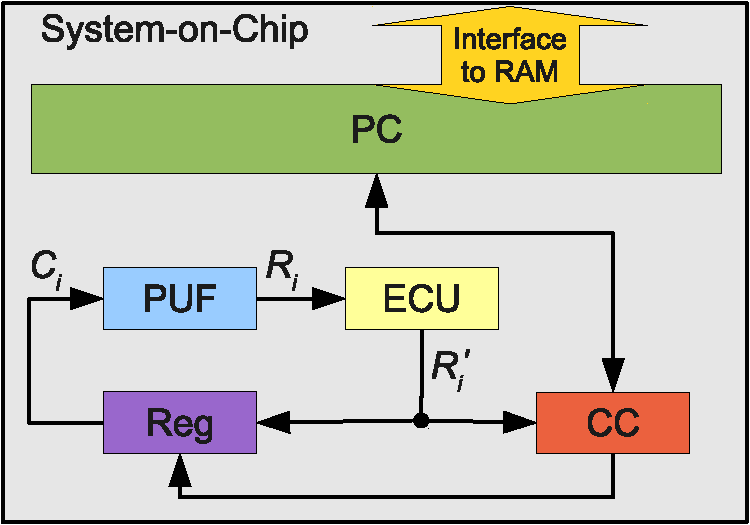
\includegraphics[width=400px]{images/rok_soc.pdf}
\label{fig:basicrok}
\caption{Block level view of a basic PUF ROK device}
\vspace{-20pt}
\end{figure}
\FloatBarrier

Note that the CC uses the error corrected PUF response to derive a key, but does not use it as a key directly.	Typically
a hash algorithm is applied to the key first. This prevents the PUF from potentially being modeled, as described in
Chapter~\ref{chapter:pufoverview}.

\subsection{PUF ROKs as a Physical System}
Because of their nature, PUF ROKs would be considered a peripheral physical system. This is because they rely
on an interaction between themselves and a computer to augment the functionality of the computer; 
they do not necessarily interact with the world just by themselves.

As a peripheral physical system, the PUF ROK must be resilient against various types of environmental attacks, such
as freezing and power analysis, as discussed in the next section, but they also must be very aware of the
interactions they have with a host system and the dangers that can pose.

\section{Security Considerations}
For our security analysis, we consider the case of a probabilistic polynomial-time (PPT) attacker $\mathcal{A}$,
with two goals.  First, the goal of $\mathcal{A}$ is to recover just the key used to encrypt or decrypt a
single message.  The second goal considered is to model the PUF, which would enable the attacker to emulate
the PUF ROK in software, thereby negating the hardware ROK guarantee.  Initially, in both cases, we assume
the adversary is capable of (at most) eavesdropping on bus communication.  That is, the adversary is unable
to observe communication between the cores in the SoC design.

Under this model, $\mathcal{A}$ is able to observe the data passing between the PC and memory, or between
the PC and a network.  Observe, though, that these messages consist exclusively of the plaintext $m$ and the
encrypted $e(m)$.  Thus, the attack is a known-plaintext attack.  However, this information offers no
additional knowledge to $\mathcal{A}$.  Even if $\mathcal{A}$ managed to reconstruct the key $\mathcal{K}$
(with negligible probability under the PPT model), this key is never used again.

The only use of reconstructing $\mathcal{K}$ in this manner is to attempt to reverse engineer
the behavior of the PUF.  However, recall that our design involved hashing the PUF output when
creating the keys.  Consequently, $\mathcal{K}$ = {\sf H}$(R_i)$, where {\sf H} is a robust cryptographic
hash function.  As a result, $\mathcal{A}$ again has only a negligible probability of reconstructing $R_i$.
Yet, we can take this analysis even further, because $R_i$ by itself is useless.  That is, $\mathcal{A}$
would also need to know the corresponding $C_i$ (or $R_{i+1}$) to begin to model the PUF.  Thus, $\mathcal{A}$
would have to accomplish a minimum of \emph{four} feats, each of which has only a negligible probability of
occurring.  Thus, we do not find such an attack to be feasible.

To continue the analysis, we loosen our assumed restrictions and grant $\mathcal{A}$ the ability to probe
inside the SoC and observe all data transferred between the cores.  Clearly, such an adversary would
succeed, as the data passed between the PUF and the CC occurs in the open.  However, this attack model
is so extreme that only the most dedicated and motivated adversaries would undertake such a task.
Similarly, users who are faced with such powerful adversaries are likely to have extensive resources 
themselves.  Thus, these users are likely to shield the processor using known tamper-resistance
techniques, and we find this threat to be minimal.

Moving away from the PPT model, we can return to the discussion of fault
injection~\cite{rsapub,pertrsa,insecrsa,rsaltr,fault} and freezing~\cite{freezing}
attacks.  Fault injection attacks fail to threaten the confidentiality of the system,
because these attacks are based on repeatedly inducing the fault with the same key.  However, PUF ROKs can
only be used once.  At best, a fault injection would become a denial-of-service, as the key would not
correctly encrypt or decrypt the message.  Freezing attacks are similarly unsuccessful, because they operate
on the assumption that the key existed in addressable memory at some point.  However, that is not the case
with PUF ROKs.  These keys are generated dynamically and are never explicitly stored outside the processor
itself.  Thus, PUF ROKs offer robust defenses against these physical attacks.

One final class of attacks to consider is power analysis~\cite{dpa}.  Simple power analysis (SPA) involves
monitoring the system's power fluctuation to differentiate between portions of cryptographic algorithms.
This information leakage can reveal how long, for instance, a modular exponentiation takes, which reveals
information about the key itself.  Differential power analysis (DPA) observes the power fluctuations over
time by repeatedly executing the cryptographic algorithm \emph{with the targeted key}.  Ironically, DPA
is considered harder to defend against than SPA.  And yet, PUF ROKs are immune to DPA (since repeated execution
is not allowed) while vulnerable to SPA.  Even though SPA is a potential threat, known techniques can prevent
these attacks~\cite{sidechan}.

\section{Out of Order Execution}
One limitation of the basic PUF ROK design in~\ref{fig:basicrok} is that it does not allow out of order execution. That is,
if five messages are encrypted and then the third is requested to be decrypted, the PUF ROK must be re-seeded, the PUF
cycled twice, and then the third cycle can be used to actually perform the decryption. To decrypt the first message, the
PUF would again need to be re-seeded. 

Supposing this had to be done many times, this process would quickly become cumbersome. As such, it is desirable to
have a PUF ROK system that allows out of order execution. Figure~\ref{fig:rok} shows the block level design for a PUF
ROK that allows this out of order execution.

\begin{figure}[!ht]
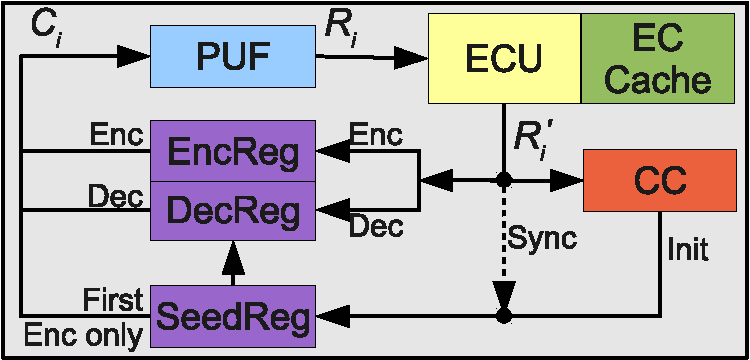
\includegraphics[width=400px]{images/rok_socreg.pdf}
\label{fig:rok}
\caption{Block level view of a PUF ROK allowing out of order execution}
\vspace{-20pt}
\end{figure}
\FloatBarrier

The modified PUF ROK is able to perform out of order executions by replacing the one original register with three
new registers, a seed register, an encryption register, and a decryption register. A cache is added to the error
correction unit as well. Note that all these new components are still internal to the PUF ROK design, so that no
buses are exposed externally.
The new design requires a new parameter, $N$. This parameter specifies the number of keys that will be stored in
the error correcting cache. The PUF ROK can then perform out of order execution on up to $N$ different keys.
The new design also introduces the Sync action, which is used to update the seed register and is further described
below.

Upon the initial seeding of the PUF ROK, the seed value is stored in the seed register. When the first encryption
is requested, the seed register is fed into the PUF. The response is then passed through error correction and stored
in both the error correcting cache as well as the encryption register. Note that the seed register is not updated here.
Upon request for another encryption, the contents of the encryption register will be used, rather than the seed register.

Upon a request for a decryption, if the requested key is still marked as valid in the error correcting cache,
the seed register is copied into the decryption register. The PUF is then cycled
and writes back to the decryption register enough times for the proper response to be obtained. Note that the
error correcting unit is correcting any potential errors after each cycling of the PUF. At the conclusion of this, the
requested key is marked as used in the error correcting cache, meaning the PUF ROK will not use it again.

Because the error correcting cache has a finite amount of space, it will be necessary to clear the cache from time to
time. This is done using the Sync action. Sync is triggered when the first key in the cache has been marked as invalid.
(Note that this first key will be associated with the value currently in the seed register.) Since the values are invalid,
this means that they will never be used again, so the value in the seed register is obsolete and can be updated.
The error correction cache thus takes control of the feedback loop. It decides which key is the last used, and then cycles
the PUF, using the contents of the seed register that many times and writing the results back into the seed register.
For example, if there are 4 values stored in the cache and values 1 and 2 are invalid, the PUF will be cycled twice,
with the resulting response being written into the seed register.

\section{Implementation}
For a prototype implementation, the Saxo-L board from KNJN.com was used.~\cite{KNJN} It contains an Altera
Cyclone FPGA and an NXP LPC2132 ARM processor. The two chips are connected together by a Serial Peripheral
Interface (SPI). Additionally, a USB and a JTAG port are available, which makes for easy communication with the
various chips.

For the ease of development, we implemented only the PUF and the register on the FPGA and then implemented
the error correction unit, cryptography core, processor core, and other supporting computation on the ARM chip. 
When the PUF or register was needed, the ARM would issue a request over the SPI link to access the appropriate component.
Figure ~\ref{fig:rokimpl} shows details of the implementation graphically.

\begin{figure}[!ht]
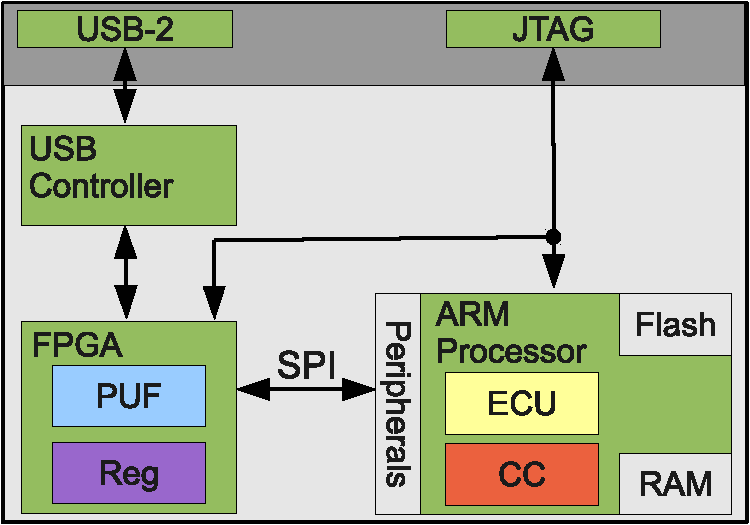
\includegraphics[width=400px]{images/rok.pdf}
\label{fig:rokimpl}
\caption{Implementation of a ROK device}
\vspace{-20pt}
\end{figure}
\FloatBarrier

The Saxo-L board is 44 x 60 mm, which makes it very portable. A production quality device would likely be smaller.
This would allow the ROK to be implemented as a small dongle that could be plugged into a USB port potentially.

For the software portion of the project, the PolarSSL~\cite{polarssl} library was used, which is an SSL library
specifically optimized for small microprocessors, such as the LPC2132.

\subsection{Limitations}
There are some limitations to the implementation, since it is simply a prototype. The fact that the SPI bus is exposed
is a huge problem. As it currently exists, an attacker could simply attach logic probes to the bus and intercept or
modify any traffic between the FPGA and ARM chip. As such, he would be able to manipulate the values of the register
as well as what the error correction unit receives. Clearly, this is not a good thing.

This vulnerability could be mitigated by using some sort of tamper proofing, such as potting, but this is a relatively
expensive solution. Instead, the ideal solution would be to incorporate all the different components on one chip, as
shown in the original design. There are soft core ARM processors available which can be instantiated on an FPGA
already. It would be possible to simply move the entire ARM processor onto the same chip as the PUF and register.
Not only would this be more secure, but it would most likely be less expensive to manufacture a device with only
one chip, rather than two.

There are a variety of soft core microprocessors available, depending on the brand of FPGA selected, so there are
alternatives available to the ARM architecture.

\subsection{Results}
Our PUF design consisted of 32 1-bit ring oscillator PUFs.
Each of these circuits consisted of a ring oscillator constructed from 37 inverting gates.
In our experiments, we found that using fewer than 37 gates yielded less consistency in the
PUF behavior.  That is, smaller PUFs increase the number of bit errors that must be corrected.
The output from the ring oscillators was linked to 20-bit
counters that were controlled by a 16-bit timer.  The timer was synchronized with a 24 MHz
clock, indicating that the timer would expire (as a result of an overflow) after 2.73 ms.
When the timer expires, the values in the counters are compared, producing a 1 or 0 depending
on which counter had the higher value.
This design used 2060 of the 2910 (71\%) logic cells available on the FPGA.  Each execution
of the PUF produced 32 bits of output.  Consequently, to generate larger keys, the ARM processor
polled the PUF multiple times, caching the result until the key size was met.

To put the performance of the PUF into perspective, we compared the execution time with measurements~\cite{nxp}
reported by NXP, the device manufacturer.  Some of NXP's measurements are reported in Figure~\ref{fig:aes}.
As each PUF execution (producing 32 bits of output) requires 2.73 ms to overflow
the timer, it is slower than encrypting one kB of data in AES.  Observe, though, that larger PUFs would
still only require 2.73 ms.  Consequently, the overhead of executing the PUF can remain small, especially
as large amounts of data are encrypted or decrypted.

%\begin{figure}[ht]
\begin{table}[!ht]
\vspace{-10pt}
\caption{NXP cryptographic measurements}
\begin{center}
\begin{tabular}{l | c c l | c}

Symmetric 	& Time		& ~~~	& RSA			& Time\\
Algorithm	& (ms/kB)	& ~~~	& Operation		& (s)\\
\cline{1-2}\cline{4-5}
AES-CBC		& 1.21		& ~	& 1024-bit encrypt	& 0.01 \\
AES-ECB		& 1.14 		& ~	& 1024-bit decrypt	& 0.27 \\
3DES-CBC	& 3.07		& ~	& 2048-bit encrypt	& 0.05 \\
3DES-ECB	& 3.00		& ~	& 2048-bit decrypt	& 2.13
%RSA Operation		& Time (s) \\
%\hline
%1024-bit encrypt	& 0.01 \\
%1024-bit decrypt	& 0.27 \\
%2048-bit encrypt	& 0.05 \\
%2048-bit decrypt	& 2.13
%\end{tabular}
%\caption{RSA cryptographic measurements reported by NXP (in seconds)}
\end{tabular}
\label{fig:aes}
\end{center}
\vspace{-25pt}
\end{table}
%\end{figure}

The comparison the RSA encryption and decryption is stark.  Observe that the 2.73 ms required to
execute the PUF is 27.3\% of the time to perform a 1024-bit encryption in RSA.  As the key size
increases (assuming the PUF size is increased accordingly so that only one polling is needed),
the PUF execution time becomes 0.13\% overhead for 2048-bit RSA decryption.  Thus, the performance
impact of polling the PUF during key generation is minimal.\footnote{Obviously, there is additional
work required to convert the PUF output into a usable key.  However, the precise timing of this
work is implementation-dependent, and the algorithms typically employed are significantly more
efficient than the modular exponentiation.  As such, we focus solely on the PUF measurement in
our analysis.}

